\documentclass{beamer}
\usepackage[utf8]{inputenc}

\usetheme{Madrid}
\usecolortheme{default}
\usepackage{amsmath,amssymb,amsfonts,amsthm}
\usepackage{txfonts}
\usepackage{tkz-euclide}
\usepackage{listings}
\usepackage{adjustbox}
\usepackage{array}
\usepackage{tabularx}
\usepackage{gvv}
\usepackage{lmodern}
\usepackage{circuitikz}
\usepackage{tikz}
\usepackage{graphicx}
\usepackage{caption}
\captionsetup{labelformat=empty}  % removes "Figure:"


\setbeamertemplate{page number in head/foot}[totalframenumber]

\usepackage{tcolorbox}
\tcbuselibrary{minted,breakable,xparse,skins}



\definecolor{bg}{gray}{0.95}
\DeclareTCBListing{mintedbox}{O{}m!O{}}{%
	breakable=true,
	listing engine=minted,
	listing only,
	minted language=#2,
	minted style=default,
	minted options={%
		linenos,
		gobble=0,
		breaklines=true,
		breakafter=,,
		fontsize=\small,
		numbersep=8pt,
		#1},
	boxsep=0pt,
	left skip=0pt,
	right skip=0pt,
	left=25pt,
	right=0pt,
	top=3pt,
	bottom=3pt,
	arc=5pt,
	leftrule=0pt,
	rightrule=0pt,
	bottomrule=2pt,
	toprule=2pt,
	colback=bg,
	colframe=orange!70,
	enhanced,
	overlay={%
		\begin{tcbclipinterior}
			\fill[orange!20!white] (frame.south west) rectangle ([xshift=20pt]frame.north west);
	\end{tcbclipinterior}},
	#3,
}
\lstset{
	language=C,
	basicstyle=\ttfamily\small,
	keywordstyle=\color{blue},
	stringstyle=\color{orange},
	commentstyle=\color{green!60!black},
	numbers=left,
	numberstyle=\tiny\color{gray},
	breaklines=true,
	showstringspaces=false,
}
\begin{document}

\title 
{4.11.22}
\date{October 11,2025}

\author 
{Navya Priya - EE25BTECH11045}
\graphicspath{./figs}

\frame{\titlepage}
\begin{frame}{Question}
    Find the equations of the diagonals of the parallelogram $PQRS$ whose vertices are P $\brak{4,2,-6}$, Q $\brak{5,-3,1}$, R $\brak{12,4,5}$ and S $\brak{11,9,-2}$.Use these equations to find the point of intersection of diagonals.
\end{frame}

\begin{frame}{Variables Taken}
\begin{table}[H]
\centering
\renewcommand{\arraystretch}{1}
\begin{tabular}{|m{2cm}|m{2cm}|}
\hline
  $\vec{P}$   &  $\myvec{4\\2\\-6}$ \\ \hline 
  $\vec{Q}$   &  $\myvec{5\\-3\\1}$ \\ \hline
  $\vec{R}$   &  $\myvec{12\\4\\5}$ \\ \hline
  $\vec{S}$   &  $\myvec{11\\9\\-2}$ \\ \hline
\end{tabular}
\end{table}
\end{frame}

\begin{frame}{Theoretical Solution}
The equation of the diagonal $\vec{R}-\vec{P}$ is
\begin{align}
    \vec{\text{x}}\,=\,\vec{P}\,+\,\lambda_1\brak{\vec{R}-\vec{P}}
\end{align}
The equation of the diagonal $\vec{S}-\vec{Q}$ is
\begin{align}
     \vec{\text{x}}\,=\,\vec{Q}\,+\,\lambda_2\brak{\vec{S}-\vec{Q}}
\end{align}
The centre of the parallelogram is the point of intersection of the diagonals.We solve the above two equations to find the centre using elemenetary transformations

From (1) \& (2)
\begin{align}
    \vec{P}\,+\,\lambda_1\brak{\vec{R}-\vec{P}}\,=\,\vec{Q}\,+\,\lambda_2\brak{\vec{S}-\vec{Q}}
\end{align}
\begin{align}
    \lambda_1\brak{\vec{R}-\vec{P}}\,-\,\lambda_2\brak{\vec{S}-\vec{Q}}\,=\,\vec{Q}\,-\vec{P}
\end{align}
\begin{align}
    \myvec{\vec{R}-\vec{P}&\vec{Q}-\vec{S}}\myvec{\lambda_1\\\lambda_2}\,=\,\vec{Q}\,-\vec{P}
\end{align}    
\end{frame}

\begin{frame}{Theoretical Solution}
    \begin{align}
    \myvec{8&-6\\2&-12\\11&3}\myvec{\lambda_1\\\lambda_2}\,=\,\myvec{1\\-5\\7}
\end{align}
\newpage
As there are only two variables, we consider the first two rows to compute $\lambda_1$,$\lambda_2$  
\begin{align}
    \myvec{8&-6\\2&-12}\myvec{\lambda_1\\\lambda_2}\,=\,\myvec{1\\-5}
\end{align}
Forming Augmented matrix from (7),
\begin{align}
\myaugvec{2}{8&-6&1\\2&-12&-5}
\end{align}
\end{frame}

\begin{frame}{Point of Intersection}
\begin{align}
\myaugvec{2}{8&-6&1\\2&-12&-5}\xleftrightarrow[R_2\to \frac{8}{21}R_2]{R_2\to R_2-\frac{1}{4}R_1}\myaugvec{2}{4&-3&-\frac{1}{2}\\[3pt]0&-2&-1}
\end{align}
From (9)
\begin{align}
    \lambda_2\,=\,\frac{1}{2}
\end{align}
Substituting the value of $\lambda_2$ in (2)
\begin{align}
    \vec{\text{x}}\,=\,\myvec{8\\3\\-\frac{1}{2}}
\end{align}
\begin{align*}
    \therefore \text{The point of intersection of the diagonals is} \myvec{8\\3\\-\frac{1}{2}}
\end{align*}
\end{frame}

\begin{frame}[fragile]{Code.c}
    \begin{lstlisting}
        #include <stdio.h>
// Structure for returning intersection
struct Point {
    float x;
    float y;
    float z;
};
// Function to compute intersection of diagonals
struct Point find_intersection() {
    // Coordinates of vertices
    float Px=4, Py=2, Pz=-6;
    float Qx=5, Qy=-3, Qz=1;
    float Rx=12, Ry=4, Rz=5;
    float Sx=11, Sy=9, Sz=-2;

 // Midpoints of diagonals
    struct Point O;
    O.x = (Px + Rx) / 2.0;

    \end{lstlisting}
\end{frame}

\begin{frame}[fragile]{Code.c}
    \begin{lstlisting}
    O.y = (Py + Ry) / 2.0;
    O.z = (Pz + Rz) / 2.0;
    return O;
}
// Function to print equations of diagonals
void print_equations() {
    float Px=4, Py=2, Pz=-6;
    float Qx=5, Qy=-3, Qz=1;
    float Rx=12, Ry=4, Rz=5;
    float Sx=11, Sy=9, Sz=-2;

    printf("Equation of diagonal PR: (x,y,z) = (%.1f, %.1f, %.1f) + t(%.1f, %.1f, %.1f)\\n",
           Px, Py, Pz, Rx-Px, Ry-Py, Rz-Pz);

    printf("Equation of diagonal QS: (x,y,z) = (%.1f, %.1f, %.1f) + s(%.1f, %.1f, %.1f)\\n",
           Qx, Qy, Qz, Sx-Qx, Sy-Qy, Sz-Qz);
}
    \end{lstlisting}
\end{frame}

\begin{frame}[fragile]{Call C.py}
    \begin{lstlisting}
        import ctypes
# Load the shared library
lib = ctypes.CDLL("./parallelogram.so")   # use "parallelogram.dll" on Windows
# Define struct mapping in Python
class Point(ctypes.Structure):
    fields = [("x", ctypes.c_float),
                ("y", ctypes.c_float),
                ("z", ctypes.c_float)]
# Bind function signatures
lib.find_intersection.restype = Point
lib.print_equations.restype = None
# Call C functions
lib.print_equations()
intersection = lib.find_intersection()
print(f"Intersection of diagonals: ({intersection.x}, {intersection.y}, {intersection.z})")
    \end{lstlisting}
\end{frame}

\begin{frame}[fragile]{Plot.py}
\begin{lstlisting}
    import numpy as np
import matplotlib.pyplot as plt
from mpl_toolkits.mplot3d import Axes3D

# Points
P = np.array([4, 2, -6])
Q = np.array([5, -3, 1])
R = np.array([12, 4, 5])
S = np.array([11, 9, -2])
O = (P + R) / 2   # intersection

# Diagonals
PR = np.vstack((P, R))
QS = np.vstack((Q, S))

fig = plt.figure(figsize=(10, 8))
ax = fig.add_subplot(111, projection='3d')

# Plot edges of parallelogram
 \end{lstlisting}
\end{frame}

\begin{frame}[fragile]{Plot.py}
\begin{lstlisting}
edges = [(P, Q), (Q, R), (R, S), (S, P)]
for edge in edges:
    ax.plot(*zip(*edge), color='black')
   # Plot diagonals
ax.plot(*zip(*PR), color='red', linestyle='--', label='Diagonal PR')
ax.plot(*zip(*QS), color='blue', linestyle='--', label='Diagonal QS')
# Scatter points
for pt in [P, Q, R, S]:
    ax.scatter(*pt, color='green', s=70, marker='x')
ax.scatter(*O, color='darkblue', s=100, marker='x', label="Intersection")
# Format coords for labels
def clean_coords(arr):
    return tuple(int(x) if float(x).is_integer() else round(float(x),2) for x in arr)
 # Labels placed with small offset
offset = 0.3
\end{lstlisting}
\end{frame}

\begin{frame}[fragile]{Plot.py}
\begin{lstlisting}
labels = {
    "P": (P, (offset, offset, offset)),
    "Q": (Q, (offset, offset, offset)),
    "R": (R, (offset, offset, offset))
    "S": (S, (offset, offset, offset)),
    "O": (O, (offset, offset, offset)),}
for name, (point, delta) in labels.items():
    label_pos = point + np.array(delta)
    ax.text(*label_pos, f"{name}{clean_coords(point)}",
            fontsize=11, fontweight="bold",
            color="darkblue" if name=="O" else "green",
            bbox=dict(facecolor="white", edgecolor="none", pad=2, alpha=0.8))
# Axes and title
ax.set_xlabel("X-axis")
ax.set_ylabel("Y-axis")
ax.set_zlabel("Z-axis")
ax.set_title("Parallelogram PQRS with Diagonals and Intersection")
ax.legend()
plt.show()
\end{lstlisting}
\end{frame}

\begin{frame}{Plot}
From the graph, theoretical solution matches with the computational solution.

\begin{figure}[H]
\centering
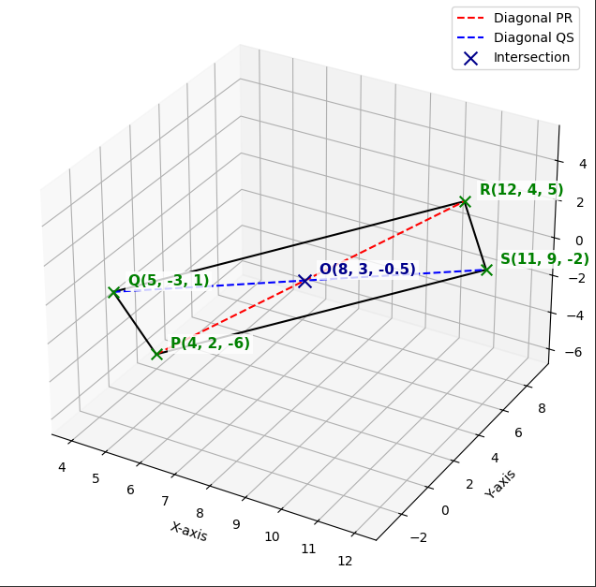
\includegraphics[width=0.5\columnwidth]{figs/graph.png}
\caption*{Parallelogram PQRS with diagonals and intersection)}
\label{fig:graph.png}
\end{figure}

    
\end{frame}
\end{document}